\section{The Qubit}
\label{sec:qubit}

The basic idea behind the implementation of a quantum device for quantum information is realizing a 2-level quantum system.
In the Quantum Device Lab this is done through superconducting circuits.
The qubits are star-shaped transmon qubits \cite{transmon_qubits}.
They are characterized by a large capacitor and a SQUID (see \cref{fig:transmon_circuit}).
The latter is flux-tunable and it is made out of two Josephson junctions in parallel.
\begin{figure}[htbp]
    \begin{minipage}[b]{0.5\linewidth}
      \centering
      


\tikzset{every picture/.style={line width=0.75pt}} %set default line width to 0.75pt        

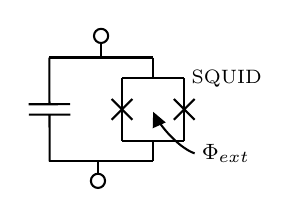
\begin{tikzpicture}[x=0.75pt,y=0.75pt,yscale=-1,xscale=1]
%uncomment if require: \path (0,97); %set diagram left start at 0, and has height of 97

%Shape: Capacitor [id:dp34366919102472526] 
\draw  [line width=0.75]  (20,23.83) -- (20.05,46.33) (30.07,51.31) -- (10.07,51.36) (30.05,46.31) -- (10.05,46.36) (20.07,51.33) -- (20.12,73.83) ;
%Straight Lines [id:da9532858123226031] 
\draw [line width=0.75]    (55,33.83) -- (85,33.83) ;
%Straight Lines [id:da4790035249190253] 
\draw [line width=0.75]    (85,33.83) -- (85,63.83) ;
%Straight Lines [id:da5192559786668693] 
\draw [line width=0.75]    (55,33.83) -- (55,63.83) ;
%Straight Lines [id:da23389027703175358] 
\draw [line width=0.75]    (55,63.83) -- (85,63.83) ;
%Straight Lines [id:da6028752523424945] 
\draw [line width=0.75]    (50,43.83) -- (60,53.83) ;
%Straight Lines [id:da22268293223346158] 
\draw [line width=0.75]    (50,53.83) -- (60,43.83) ;
%Straight Lines [id:da7666685944565205] 
\draw [line width=0.75]    (80,53.83) -- (90,43.83) ;
%Straight Lines [id:da0860971350076063] 
\draw [line width=0.75]    (80,43.83) -- (90,53.83) ;
%Straight Lines [id:da32147396047949894] 
\draw [line width=0.75]    (20,23.83) -- (70,23.83) ;
%Straight Lines [id:da3842851758264739] 
\draw [line width=0.75]    (20,73.83) -- (70,73.83) ;
%Straight Lines [id:da04257544936461244] 
\draw [line width=0.75]    (70,23.83) -- (70,33.83) ;
%Straight Lines [id:da22754146049716317] 
\draw [line width=0.75]    (70,63.83) -- (70,73.83) ;
%Straight Lines [id:da6459112049306985] 
\draw [line width=0.75]    (43.42,79.83) -- (43.42,73.83) ;
%Shape: Circle [id:dp6531205659740902] 
\draw  [line width=0.75]  (40,83.25) .. controls (40,81.36) and (41.53,79.83) .. (43.42,79.83) .. controls (45.3,79.83) and (46.83,81.36) .. (46.83,83.25) .. controls (46.83,85.14) and (45.3,86.67) .. (43.42,86.67) .. controls (41.53,86.67) and (40,85.14) .. (40,83.25) -- cycle ;
%Straight Lines [id:da42435820900303667] 
\draw [line width=0.75]    (45,16.83) -- (45,23.83) ;
%Shape: Circle [id:dp32456243319283773] 
\draw  [line width=0.75]  (48.33,13.33) .. controls (48.38,15.22) and (46.89,16.78) .. (45,16.83) .. controls (43.11,16.88) and (41.55,15.39) .. (41.5,13.5) .. controls (41.45,11.62) and (42.94,10.05) .. (44.83,10) .. controls (46.71,9.95) and (48.28,11.44) .. (48.33,13.33) -- cycle ;

%Curve Lines [id:da7487363329577509] 
\draw [color={rgb, 255:red, 0; green, 0; blue, 0 }  ,draw opacity=1 ]   (90,70) .. controls (83.25,67.65) and (75.22,59.11) .. (71.34,52.55) ;
\draw [shift={(70,50)}, rotate = 65.77] [fill={rgb, 255:red, 0; green, 0; blue, 0 }  ,fill opacity=1 ][line width=0.08]  [draw opacity=0] (7.14,-3.43) -- (0,0) -- (7.14,3.43) -- cycle    ;

% Text Node
\draw (87,33.83) node [anchor=west] [inner sep=0.75pt]   [align=left] {{\scriptsize SQUID}};
% Text Node
\draw (92,70) node [anchor=west] [inner sep=0.75pt]  [font=\footnotesize,color={rgb, 255:red, 0; green, 0; blue, 0 }  ,opacity=1 ] [align=left] {$\displaystyle \Phi _{\text{ext}}$};


\end{tikzpicture}
      \captionsetup{skip=-20pt}
      \caption{Circuit diagram of a transmon qubit}
      \label{fig:transmon_circuit}
    \end{minipage}
    \hfill
    \begin{minipage}[b]{0.45\linewidth}
      \centering
      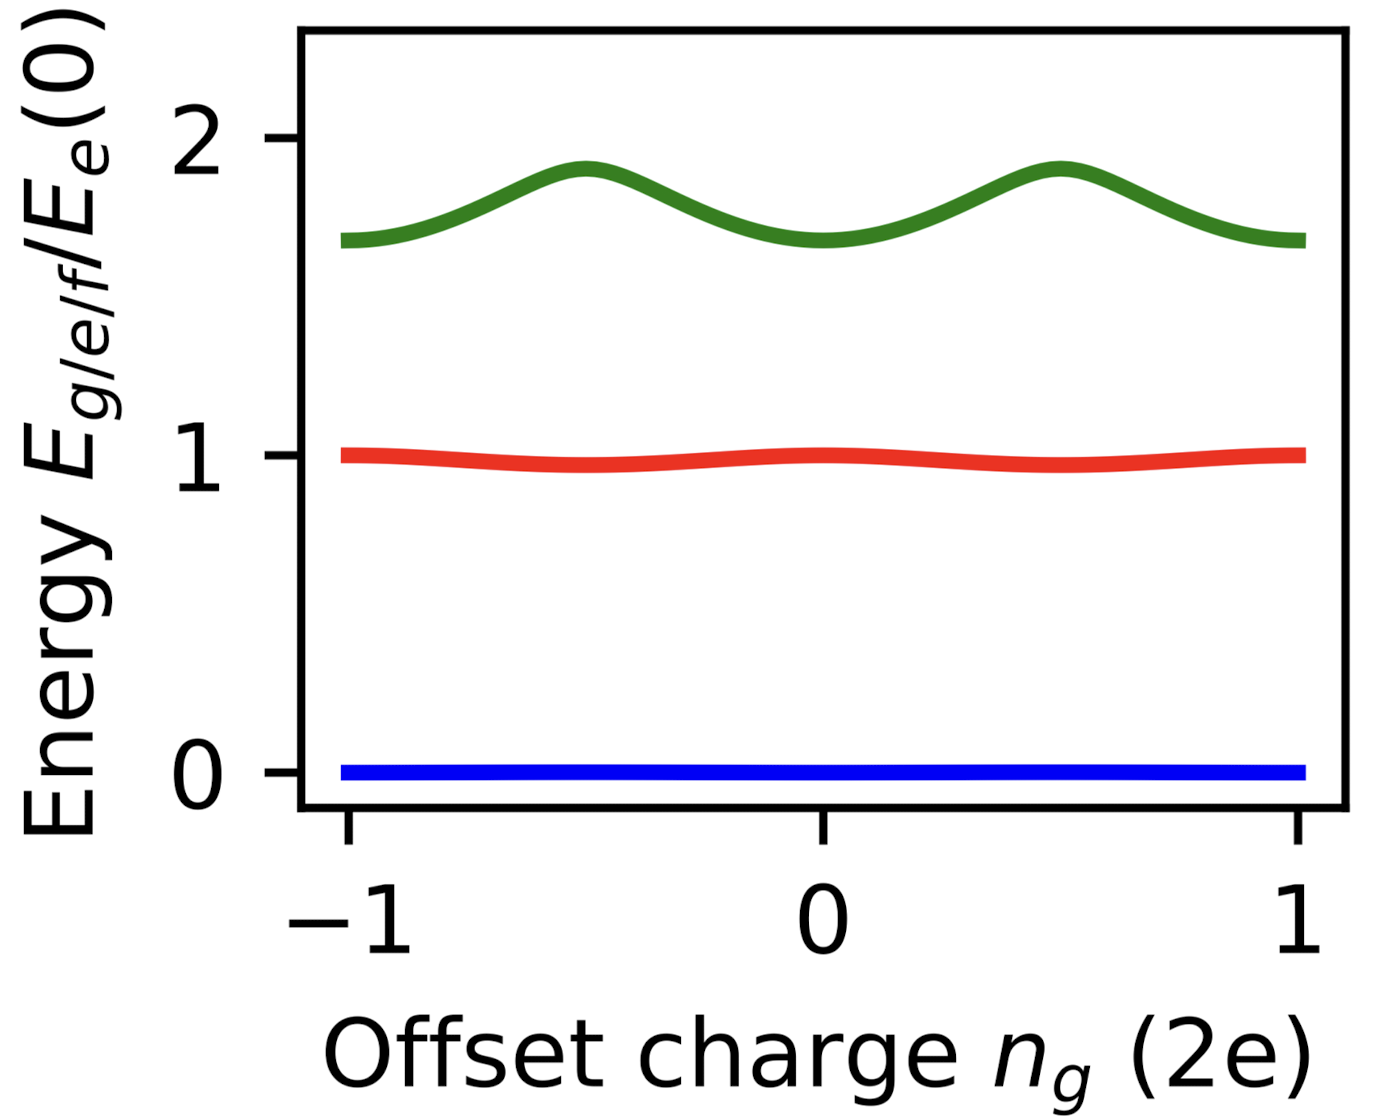
\includegraphics[width = 0.5 \textwidth]{Images/Chap1/Qubit_energy.png}
      \caption{Energy spectrum relative to $N_g$}
      \label{fig:qubit_energy}
    \end{minipage}
  \end{figure}
  

The Hamiltonian representing the dynamics of such a transmon is 
\begin{equation}
    \hat{H} = E_C (\hat{N} - N_g)^2 - E_{J_0, \text{max}} \cos(\pi\frac{\Phi_{\text{ext}}}{\Phi_0})\cos\hat{\delta}
\end{equation}
where $\hat{N}$ is the operator of number of Cooper pairs in the island and $\hat{\delta}$ is the phase operator of the transmon.
This can be seen as a non-linear harmonic oscillator.

By changing the external magnetic flux through the SQUID $\Phi_\text{ext}$, it's possible to change the energy splitting between the first two energy levels $\ket{g}$ and $\ket{e}$, and thus the frequency of the qubit.
Furthermore, the anharmonicity allows us to access the first and second transition separately, since they have different energy gaps (see \cref{fig:qubit_energy}).
Nevertheless, it is important to mention that in our particular setup the qubits are not flux-tunable, because it is not useful for out purposes.
We will present our setup in more detail in \Cref{sec:our_setup}.
The qubits are also coupled to a charge line, which is used to perform single-qubits rotations.
\begin{figure}[t]
    \centering
    \begin{subfigure}[b]{0.45\linewidth}
      \centering
      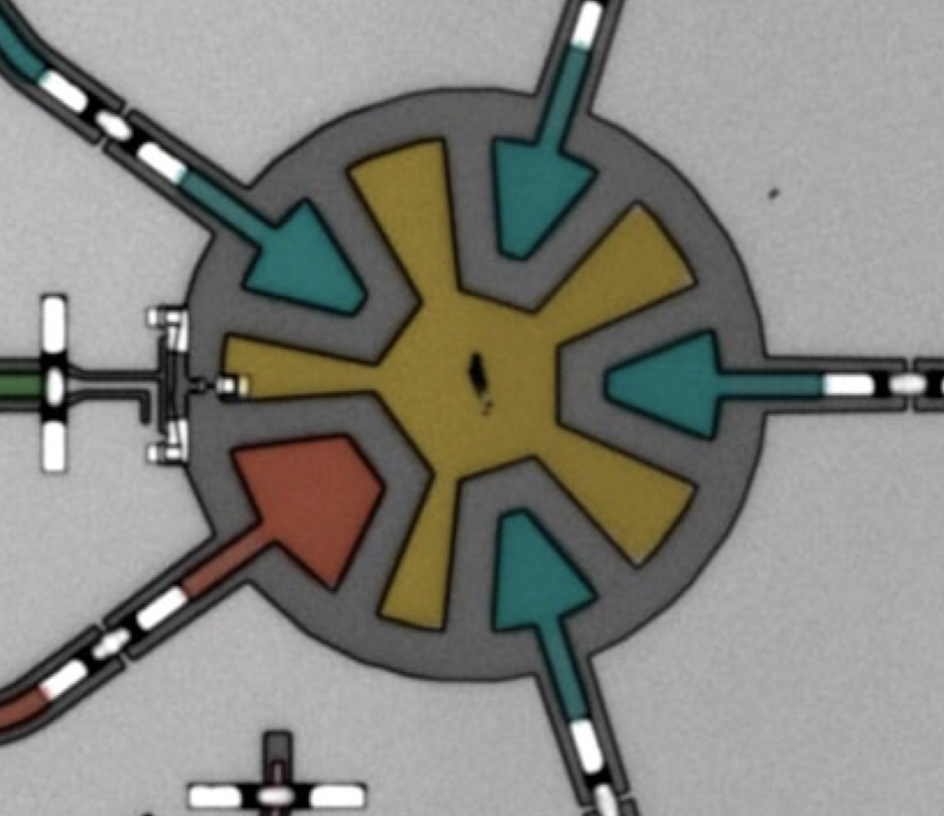
\includegraphics[height=3cm]{Images/Chap1/star_transmon.png}
      \caption{Star-shaped transmon}
      \label{fig:stqr_transmon}
    \end{subfigure}
    \hfill
    \begin{subfigure}[b]{0.45\linewidth}
      \centering
      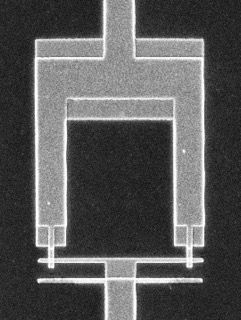
\includegraphics[height=3cm]{Images/Chap1/SQUID.jpeg}
      \caption{Zoom-in of a SQUID loop}
      \label{fig:squid_loop}
    \end{subfigure}
    \caption{Images of the devices used in the lab}
    \label{fig:transmon_squid_images}
  \end{figure}

The qubits are star-shaped and made out of niobium(see \cref{fig:transmon_squid_images}), fabricated on a silicon substrate.
